\subsection{Gradient Flow}
\label{sec:GradFlow}

The parameter-space/function-space duality described in Sec.~\ref{sec:Init} yields intersting insight
on the training process. Our main aim in this paper is understanding the dynamics driving the
training process. Therefore, we work in a simplified setting where we consider standard gradient descent
and data that depend linearly on the unknwon PDFs, as shown in Eq.~\eqref{eq:TheoryPred}. The generalization
to other minimizers and non-linear data is left to future investigations, but is expected to yield
qualitatively similar results. The results
in this subsection apply to any generic parametrization of the unknown function, they are {\em not}\
specific to the case of using NNs for the parametrization.

Gradient descent is described as a continuous flow of the parameters $\theta$ in training time $t$
along the negative gradient of the loss function $\mathcal{L}$. The parameters and the fields during
training are labelled by adding an index $t$, so that \eg\ $\theta_{t,\mu}$ identifies the parameter
$\theta_\mu$ at time $t$.
The gradient flow is given by
\begin{align}
    \label{eq:GradientFlowDef}
    \ddt &\theta_{t,\mu} = -\nabla_\mu \mathcal{L}_t\, .
\end{align}
We focus here on quadratic loss functions that are obtained as the negative logarithm of Gaussian
data distributions around their theoretical predictions,
\begin{align}
    \label{eq:QuadLoss}
    \mathcal{L}_t = \frac12 \left(Y - T[f_t]\right)^T C_Y^{-1} \left(Y - T[f_t]\right)\, ,
\end{align}
where $C_Y$ is the covariance of the data, which includes statistical and systematic errors given by
the experiments and also any theoretical error, like \eg\ missing higher orders in the theoretical
predictions. Indices that are summed over are suppressed to improve the clarity of the equations.
Note that the loss function at training time $t$ is computed using the theoretical prediction $T[f_t]$,
\ie\ the result of Eq.~\eqref{eq:TheoryPred} computed using the fields at training time $t$. For a quadratic
loss, the gradient is
\begin{align}
    \nabla_\mu \mathcal{L}_t = - \left(\nabla_\mu f_t\right)^T \left(\frac{\partial T}{\partial f}\right)_t
      C_Y^{-1} \epsilon_t\, ,
\end{align}
where, writing explicitly the data index,
\begin{align}
    \label{eq:EpsDef}
    \epsilon_{t,I} = Y_I - T_I[f_t]\, , \quad I=1, \ldots, \ndat\, .
\end{align}
For the specific case of a quadratic loss function, the gradient is proportional to $\epsilon_t$, which
is the difference between the theoretical prediction and the data at training time $t$. If at some point
during the training the theoretical predictions reproduce all the data, the training process ends.
A further simplification is obtained in the case of data that depend linearly on the unknown function $f$.
In the specific case of NNPDF fits, the integrals in Eq.~\eqref{eq:TheoryPred} are approximated by
a Riemann sum over the grid of $x$ points,
\begin{align}
    \label{eq:FKTabDef}
    T_I[f] \approx \sum_{i=1}^{\nflav}\sum_{\alpha=1}^{\ngrid} \FKtab_{Ii\alpha} f_{i\alpha}\, ,
\end{align}
and hence
\begin{align}
    \label{eq:dTbydf}
    \left(\frac{\partial T_I}{\partial f_{i\alpha}}\right)_t =
        \FKtab_{Ii\alpha}\, ,
\end{align}
and is independent of $t$. The flow of parameters $\theta$ translates into a flow for the fields,
\begin{align}
    \label{eq:NTKFlow}
    \ddt &f_{t,i_1\alpha_1} = (\nabla_\mu f_{t,i_1\alpha_1}) \ddt \theta_\mu =
      \Theta_{t,i_1\alpha_1i_2\alpha_2}
      \FKtabT_{i_2\alpha_2I} \left(C_Y^{-1}\right)_{IJ} \epsilon_{t,J}\, ,
\end{align}
where
\begin{align}
    \label{eq:NTKDef}
    \Theta_{t,i_1\alpha_1i_2\alpha_2} = \sum_\mu
    \nabla_\mu f_{t,i_1\alpha_1} \nabla_\mu f_{t,i_2\alpha_2}\, .
\end{align}
For clarity, we often omit indices and write
\begin{align}
    \label{eq:dTdfForLinearObs}
    \left(\frac{\partial T}{\partial f}\right)_t
        &= \FKtab\, , \\
    \label{eq:NTKDefNoIndices}
    \Theta_t
        &= \left(\nabla_\mu f_t\right) \left(\nabla_\mu f_t\right)^T\, , \\
    \label{eq:FlowEquationNoIndices}
    \ddt f_t
        &= \Theta_t \FKtabT C_Y^{-1} \epsilon_t\, .
\end{align}
Note that these equations do not refer to a specific parametrization and remain valid when some
explicit functional form is chosen to parametrize the PDFs, as \eg\ in
Refs.~\cite{Bailey:2020ooq,Hou:2019efy}.

\subsection{Lazy Training for the Flow Equation}
\label{sec:Lazy}

The large-$n_{\ell}$ effective theory discussed in Sect.~\ref{sec:Init} also predicts that
the NTK remains constant along training, up to corrections that are $O(1/n_{\ell})$, see
Ref.~\cite{DBLP:journals/corr/abs-1806-07572} and references therein for a derivation of this result.
This regime is sometimes referred to as {\em lazy kernel training}, and allows an analytical
solution of the flow equation. In this section, we discuss the analytical solution, which allows us 
to write an explicit expression for the trained field as a function of the field at initialization and the data. 
The applicability of these expressions to the case of the trained NNPDF networks is discussed in 
Sects.~\ref{sec:NTKPheno} and~\ref{sec:TrainClosure}.

We start by rewriting Eq.~\eqref{eq:FlowEquationNoIndices} as
\begin{align}
    \label{eq:FlowEqTwo}
    \ddt f_t = -\Theta M f_t + b\, ,
\end{align}
where
\begin{align}
    M &= \FKtabT C_Y^{-1} \FKtab\, , \quad b = \Theta \FKtabT C_Y^{-1} Y\, .
\end{align}
The eigenvectors of $\Theta$,
\begin{align}
    \label{eq:ThetaEigensystem}
    \Theta z^{(k)} = \lambda^{(k)} z^{(k)}\, ,
\end{align}
provide a basis for expanding Eq.~\eqref{eq:FlowEqTwo}. It is necessary at this stage to distinguish
the components of $f_t$ that are in the kernel of $\Theta$ from the ones that are in the orthogonal
complement, hence we introduce the notation
~\footnote{
    The scalar product is defined as
    \[
        \left(f'_{t'}, f_t\right)
            = \sum_{i,\alpha} f'_{t',i\alpha} f_{t,i\alpha}\, .
    \]
}
\begin{align}
    \label{eq:ParallelCompnents}
    &f^\parallel_{t,k} = \left(z^{(k)}, f_t\right)\, , \quad \text{if}\ \lambda^{(k)} = 0\, , \\
    \label{eq:OrthogonalComponents}
    &f^\perp_{t,k} = \frac{1}{\sqrt{\lambda^{(k)}}} \left(z^{(k)}, f_t\right)\, , \quad
        \text{if}\ \lambda^{(k)} \neq 0\, .
\end{align}
One can readily see that the components in the kernel of $\Theta$, $\text{ker}\ \Theta$,
do not evolve during the flow,
\begin{align}
    \label{eq:FlowParallel}
    \ddt f^\parallel_{t,k} = 0
        \quad \Longrightarrow \quad f^\parallel_{t,k} = f^\parallel_{0,k}\, .
\end{align}
The flow equation for the orthogonal components can be written as
\begin{align}
    \label{eq:FlowPerp}
    \ddt f^\perp_{t,k} = - H^\perp_{kk'} f^\perp_{t,k'}
        + B^\perp_{k}\, ,
\end{align}
where the indices on quantities that have a $\perp$ suffix only span the space orthogonal to the kernel
of $\Theta$, while the indices on quantities that have a $\parallel$ suffix span the kernel.
In Eq.~\eqref{eq:FlowPerp}, we introduced
\begin{align}
    H^\perp_{kk'} &= \sqrt{\lambda^{(k)}} \left(z^{(k)}, M z^{(k')}\right) \sqrt{\lambda^{(k')}}\, ,\\
    B^\perp_k &= -\sqrt{\lambda^{(k)}} \left[\left(z^{(k)}, M z^{(k')}\right) f^\parallel_{0,k'}
        - \left(z^{(k)}, \FKtabT C_Y^{-1} Y\right)\right]\, .
\end{align}
We refer to $H^\perp$ as the flow (or training) Hamiltonian; we see explicitly in the definition above that
the flow dynamics is determined by a combination of the architecture of the NN, encoded in the NTK, and the
data, on which $M$ depends. More specifically, the matrix elements of $M$ can be written as
\begin{align}
    \label{eq:MMatElems}
    \left(z^{(k)}, M z^{(k')}\right) = T^{(k)T} C_Y^{-1} T^{(k')}\, ,
\end{align}
where $T^{(k)} = T[z^{(k)}]$ is the vector of theory predictions for the data obtained using $z^{(k)}$ as the
input PDF. Similarly, we have
\begin{align}
    \label{eq:BMatElems}
    \left(z^{(k)}, \FKtabT C_Y^{-1} Y\right) = T^{(k)T} C_Y^{-1} Y\, .
\end{align}
Denoting by $d^\perp$ the dimension of the subspace orthogonal to $\text{ker}\ \Theta$, $H^\perp$ is
a $d^\perp\times d^\perp$ symmetric matrix, whose eigenvalues and eigenvectors satisfy
\begin{align}
    H^\perp_{kk'} w^{(i)}_{k'} = h^{(i)} w^{(i)}_{k}\, .
\end{align}
The solution to Eq.~\eqref{eq:FlowPerp} can be written as the sum of the solution of the
homogeneous equation, $\hat{f}^{\perp}_{t,k}$, and a particular solution of the full equation.
The solution of the homogeneous equation is
\begin{align}
    \label{eq:HomoSoln}
    \hat{f}^{\perp}_{t,k} = \sum_{i=1}^{d^\perp} f^{\perp}_{0,i} e^{-h^{(i)}t} w^{(i)}_k\, ,
\end{align}
where
% ~\footnote{
%     Note that here the scalar product is computed in the subspace orthogonal to the kernel of $\Theta$,
%     \[
%         \left(w^{(i)}, f^\perp_0\right) = \sum_{k=1}^{d_\perp} w^{(i)}_{k} f^\perp_{0,k}
%     \]
% }
\begin{align}
    \label{eq:InitialCi}
    f^{\perp}_{0,i} = \sum_{k=1}^{d_\perp} w^{(i)}_k f^\perp_{0,k}\, ,
        %= \left(w^{(i)}, f^\perp_0\right)\, ,
\end{align}
guarantees that the initial condition $\hat{f}^\perp_{t,k}=f^\perp_{0,k}$ is
satisfied. Similarly, if we define
\begin{align}
    \label{eq:BiDef}
    \Upsilon^{(i)} = \sum_{k=1}^{d_\perp} w^{(i)}_k B^\perp_{k}\, ,
        %= \left(w^{(i)}, B^\perp\right)\, ,
\end{align}
then
\begin{align}
    \label{eq:PartSol}
    \check{f}^\perp_{t,k} = \sideset{}{'}\sum_{i} \frac{1}{h^{(i)}} \Upsilon^{(i)}
        \left(1 - e^{-h^{(i)}t}\right) w^{(i)}_k\, ,
\end{align}
where the sum only involves the non-zero modes of $H^\perp$,
is a particular solution of the inhomogeneous equation, which satisfies the boundary
condition $\check{f}^{\perp}_{0,k}=0$. Finally, the solution of the flow equation in the subspace orthogonal to
$\text{ker}\ \Theta$ is
\begin{align}
    f^\perp_{t,k}
    \label{eq:FlowSolution}
        &= \hat{f}^\perp_{t,k} + \check{f}^\perp_{t,k}
        % &= \sum_{i=1}^{d^\perp}  \left(w^{(i)}, f^\perp_0\right) e^{-h^{(i)}t} w^{(i)}_k
        %     + \sideset{}{'}\sum_{i=1}  \frac{1}{h^{(i)}} \left(w^{(i)}, B^\perp\right)
        %         \left(1 - e^{-h^{(i)}t}\right) w^{(i)}_k
        \, .
\end{align}
Collecting all terms yields a simple (and useful!) expression,
\begin{align}
    \label{eq:AnalyticSol}
    f_{t,\alpha}
        = U(t)_{\alpha\alpha'} f_{0,\alpha'} + V(t)_{\alpha I} Y_{I}\, .
\end{align}
The two evolution operators $U(t)$ and $V(t)$ have lengthy, yet explicit, expressions, which we
summarise here: 
\begin{align}
    U(t)_{\alpha\alpha'} = \hat{U}^\perp(t)_{\alpha\alpha'}
        + \check{U}^\perp(t)_{\alpha\alpha'} + U^\parallel_{\alpha\alpha'}\, ,
\end{align}
where
\begin{align}
    \hat{U}^\perp(t)_{\alpha\alpha'}
        = \sum_{k,k'\in\perp} \sqrt{\lambda^{(k)}} z^{(k)}_\alpha 
            \left[\sum_i w^{(i)}_{k} e^{-h^{(i)}t} w^{(i)}_{k'}\right]
            z^{(k')}_{\alpha'} \frac{1}{\sqrt{\lambda^{(k')}}}\, ,
\end{align}
and
\begin{align}
    U^\parallel_{\alpha\alpha'}
        = \sum_{k''\in\parallel} z^{(k)}_\alpha z^{(k)}_{\alpha'} \, .
\end{align}
The contributions from $\check{U}^\perp(t)$ and $V(t)$ are more easily expressed by
introducing the operator
\begin{align}
    \label{eq:MOperatorDef}
    \mathcal{M}(t)_{\alpha\alpha'} 
        = \sum_{k,k'\in\perp} \sqrt{\lambda^{(k)}} z^{(k)}_\alpha 
            \left[\sideset{}{'}\sum_{i} w^{(i)}_{k} \frac{1}{h^{(i)}}\, 
            \left( 1- e^{-h^{(i)}t}\right) w^{(i)}_{k'}\right]
            z^{(k')}_{\alpha'} \sqrt{\lambda^{(k')}}\,. 
\end{align}
Then, we can write
\begin{align}
    \label{eq:UperpCheck}
    \check{U}^\perp(t)
        = - \mathcal{M}(t)\; \FKtabT C_Y^{-1} \FKtab 
            \left[\sum_{k''\in\parallel} z^{(k'')} z^{(k'') T}\right]\, ,
\end{align}
and
\begin{align}
    V(t) = \mathcal{M}(t)\; \FKtabT C_Y^{-1}\, ,
\end{align}
where we note that the term in the bracket in Eq.~\eqref{eq:UperpCheck} is simply the projector on the 
kernel of the NTK. 

\paragraph{Physical Interpretation.} \ac{Check the discussion below} The four terms that appear in the analytical solution have a clear physical interpretation. 
\begin{itemize}
    \item The first term $\hat{U}^\perp(t)$ suppresses the components of the initial condition that lie in the subspace orthogonal 
    to the kernel of the NTK. These are the components that are learned by the network during training. While the trained solution
    still depends on its value at initialization, that dependence is suppressed during training. This suppression 
    is exponential in the training time, and the rates are given by the eigenvalues of 
    $H^{\perp}$.
    \item The contribution from $U^\parallel$ yields the component of the initial condition that lies in the kernel of the NTK. 
    As such, those components remain unchanged during training and are part of the trained field at all times $t$. 
    \item The two remaining contributions are best understood by combining them together,
    \begin{align}
        \label{eq:DataCorrectedInference}
        \check{U}^{\perp}(t) f_{0} + V(t) Y 
            = \mathcal{M}(t)\; \FKtabT C_Y^{-1} \left[Y - \FKtab f_{0}^{\parallel}\right]\, .
    \end{align}
    The parallel component of the initial condition $f_{0}^{\parallel}$ does not evolve during training, and therefore it yields
    a contribution $\FKtab f_{0}^{\parallel}$ to the theoretical prediction of the data points at all times $t$. This is 
    taken into account by subtracting this
    contribution from the data, before the inference is performed.
\end{itemize}

% Collecting all terms yields a simple (and useful!) expression,
% \begin{align}
%     \label{eq:AnalyticSol}
%     f_{t,\alpha}
%         = U(t)_{\alpha\alpha'} f_{0,\alpha'} + V(t)_{\alpha I} Y_{I}\, .
% \end{align}
% The two evolution operators $U(t)$ and $V(t)$ have lengthy, yet explicit, expressions, which we
% summarise here or move to an appendix: \ac{$U^\parallel$ should not be time-dependent, right?}
% \begin{align}
%     U(t)_{\alpha\alpha'} = \hat{U}^\perp(t)_{\alpha\alpha'}
%         + \check{U}^\perp(t)_{\alpha\alpha'} + U^\parallel_{\alpha\alpha'}\, ,
% \end{align}
% where
% \begin{align}
%     \hat{U}^\perp(t)_{\alpha\alpha'}
%         &= \sum_i Z^{(i)}_{\alpha} e^{-h^{(i)}t} Z^{(i)}_{\alpha'}\, , \\
%     Z^{(i)}_{\alpha}
%         &= \sum_{k\in\perp} \sqrt{\lambda^{(k)}} z^{(k)}_\alpha w^{(i)}_{k}\, ,
% \end{align}
% and
% \begin{align}
%     \check{U}^\perp(t)_{\alpha\alpha'}
%         &= \sideset{}{'}\sum_{i} Z^{(i)}_{\alpha} \frac{1}{h^{(i)}} \left(1 - e^{-h^{(i)}t}\right) \tilde{Z}^{(i)}_{\alpha'}\, , \\
%     \tilde{Z}^{(i)}_{\alpha}
%         &= -\sum_{k'\in\perp} \sum_{k''\in\parallel} w^{(i)}_{k'} \sqrt{\lambda^{(k')}}
%             T^{(k') T} C_Y^{-1} T^{(k'')} z^{(k'')}_{\alpha}\, ,
% \end{align}
% and
% \begin{align}
%     U^\parallel_{\alpha\alpha'}
%         = \sum_{k\in\parallel} z^{(k)}_\alpha z^{(k)}_{\alpha'} \, ,
% \end{align}
% and
% \begin{align}
%     V(t)_{\alpha I} = \sideset{}{'}\sum_{i} Z^{(i)}_{\alpha} \frac{1}{h^{(i)}} \left(1 - e^{-h^{(i)}t}\right)
%         \tilde{T}^{(i)}_{I}\, ,
% \end{align}
% and
% \begin{align}
%     \tilde{T}^{(i)}_{I} = \sum_{k'\in\perp} w^{(i)}_{k'} \sqrt{\lambda^{(k')}}
%         T^{(k')}_J \left(C_Y^{-1}\right)_{JI}\, .
% \end{align}

\subsection{Behaviour of the solution}
\label{sec:BehaviourOfSolution}
The solution in Eq.~\eqref{eq:AnalyticSol} is the main result of this section. It shows that the
training process can be described as the sum of a linear transformation of the initial fields $f_{0,\alpha}$,
which are the preactivations of the output layer at initialization, and a linear transformation
of the data $Y_I$. The two transformations depend on the flow time $t$ and are given by the evolution
operators $U(t)$ and $V(t)$. Eq.~\eqref{eq:AnalyticSol} encode the information on the central value
and the variance of the trained fields, and any other quantity that is derived from the PDFs. 

\subsubsection{Central value of the trained fields}
\label{sec:CentralValue}
The central values of the trained fields is obtained by taking the expectation value of
Eq.~\eqref{eq:AnalyticSol} over the initial fields, which are approximately Gaussian distributed at 
initialization, and over the fluctuations of the NTK,
\begin{align}
    \label{eq:MeanValAtT}
    \bar{f}_{t,\alpha} = \mathbb{E}\left[f_{t,\alpha}\right]
        = \mathbb{E}\left[U(t)_{\alpha\alpha'} f_{0,\alpha'}\right]
            + \mathbb{E}\left[V(t)_{\alpha I} Y_I\right] \, .
\end{align}
Note that the first term on the right-hand side of Eq.~\eqref{eq:MeanValAtT} can only be non-zero because of the
correlations between $U(t)$ and $f_0$. In the absence of such correlations, the first term would be given by the product
of the expectation values and hence would vanish up to corrections of order $\mathcal{O}(1/n)$, since the expectation
value of the fields at initialization vanishes in the limit of infinitely wide networks.
Assuming that the correlations between the initial fields and the evolution operators vanish, we can write
\begin{align}
    \label{eq:MeanUt}
    \bar{U}(t)
        &= \mathbb{E}\left[U(t)\right]\, , \\
    \label{eq:MeanVt}
    \bar{V}(t)
        &= \mathbb{E}\left[V(t)\right]\, ,
\end{align}
and
\begin{equation}
    \label{eq:MeanValAtTNoCorr}
    \bar{f}_{t,\alpha} = \bar{U}(t)_{\alpha\alpha'} \bar{f}_{0,\alpha'}
        + \bar{V}(t)_{\alpha I} Y_I = \bar{V}(t)_{\alpha I} Y_I \, .
\end{equation}

The second term in Eq.~\eqref{eq:MeanValAtT}, or equivalently Eq.~\eqref{eq:MeanValAtTNoCorr}, explicitly shows the contribution
of each data point to the central value of the
trained fields at each value of $x_{\alpha}$. It is worthwhile remarking that in this limit, the central value
from the set of trained networks is a linear combination of the data points, with coefficients given by the
evolution operator $V(t)_{\alpha I}$. In this respect, the trained NNs behave like other well-known linear methods for 
solving inverse problems, like \eg\ Backus-Gilbert or Gaussian Processes. It is interesting to compare the matrix $V(t)$ with 
the corresponding linear operators that enter in Backus-Gilbert or Gaussian Processes solutions. 

\paragraph{Central value at infinite training time.}

In the limit of infinite training time, the evolution operators $U(t)$ and $V(t)$ simplify and yield an 
elegant interpretation of the minimum of the cost function. For large training times, we have
\begin{align}
    \label{eq:UhatInfty}
    \hat{U}^\perp_{\infty, \alpha\alpha'}
        &= \lim_{t\to\infty}\hat{U}^\perp(t)_{\alpha\alpha'} = 0\, \\
    \label{eq:MOperatorInfty}
    \mathcal{M}_{\infty, \alpha\alpha'} 
        &= \lim_{t\to\infty}\mathcal{M}(t)_{\alpha\alpha'} = \sum_{k,k'\in\perp} \sqrt{\lambda^{(k)}} z^{(k)}_\alpha 
        \left[\sideset{}{'}\sum_{i} w^{(i)}_{k} \frac{1}{h^{(i)}}\, 
        w^{(i)}_{k'}\right] z^{(k')}_{\alpha'} \frac{1}{\sqrt{\lambda^{(k')}}}\, ,
\end{align}
and explicit expressions for $\check{U}^\perp_{\infty}$ and $V_{\infty}$ are obtained from $\mathcal{M}_{\infty}$.
The term in the square bracket in Eq.~\eqref{eq:MOperatorInfty} is the spectral decomposition of the pseudoinverse 
of $H^\perp$ in $d_\perp$ orthogonal subspace. So, the operator $\mathcal{M}_{\infty}$ acts as follow on a field 
$f_{\alpha}$:
\begin{enumerate}
    \item The term on the right of the square bracket computes the coordinate $f_k$ introduced in 
    Eq.~\eqref{eq:OrthogonalComponents}. The $f_k$ are a set of coordinates for the component $f^\perp$ 
    of the field that evolves during training, 
    \begin{align}
        \label{eq:RightOfTheBracket}
        f^\perp = \sum_{k\in\perp} \sqrt{\lambda^{(k)}} f_k\, z^{(k)}\,  .
    \end{align}
    \item The term in the square bracket applies the pseudoinverse to the coordinates $f_k$, 
    \begin{align}
        \label{eq:ApplyPseudoInv}
        f'_k = \left(H^\perp\right)^+_{kk'} f_{k'}\, .
    \end{align}
    \item The final term on the left of the square bracket reconstructs the full field corresponding to the modified 
    $f'_{k}$,
    \begin{align}
        \label{eq:LeftOfTheBracket}
        f^{'\perp} = \sum_{k\in\perp} \sqrt{\lambda^{(k)}} f'_{k}\, z^{(k)}\, .
    \end{align}
    
\end{enumerate}

As discussed at the end of Sect.~\ref{sec:Lazy} it is convenient to 
combine the contributions of $\check{U}^\perp_{\infty}$ and $V_{\infty}$,
\begin{align}
    \label{eq:DataCorrectedInferenceAtInfty}
    \check{U}^{\perp}_{\infty} f_{0} + V_{\infty} Y 
        = \mathcal{M}_{\infty}\; \FKtabT C_Y^{-1} \left[Y - \FKtab f_{0}^{\parallel}\right]\, .
\end{align}
The contribution to the observables from the parallel components of $f$ does not change during training, 
therefore that contribution is subtracted from the data and the orthogonal components of $f$ are adjusted to 
minimize the $\chi^2$ of the corrected data. The minimum of the $\chi^2$ in the orthogonal subspace is found
applying $\mathcal{M}_{\infty}$, \ie\ by projecting in the orthogonal subspace, applying the pseudoinverse and 
finally recompute the full field as detailed above. 

\subsubsection{Covariance of the trained fields}
\label{sec:Covariance}
% L0
% ===================================
  \begin{figure}[ht!]
    \centering
    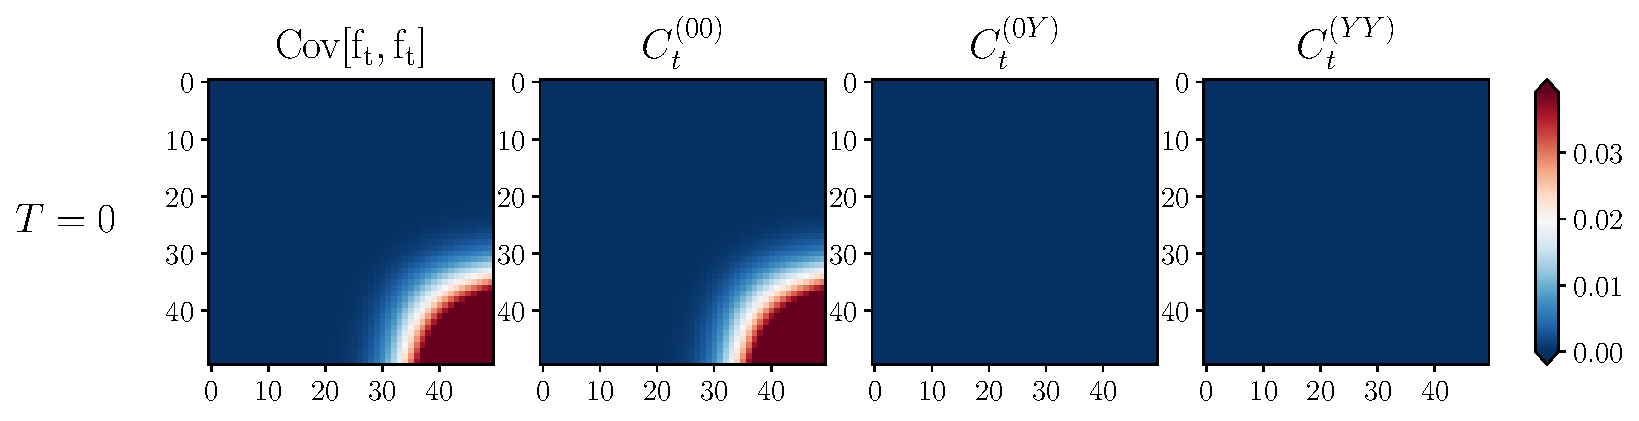
\includegraphics[width=0.90\textwidth]{plots/analytical_solution/covariance_ft_0_L0.pdf}
    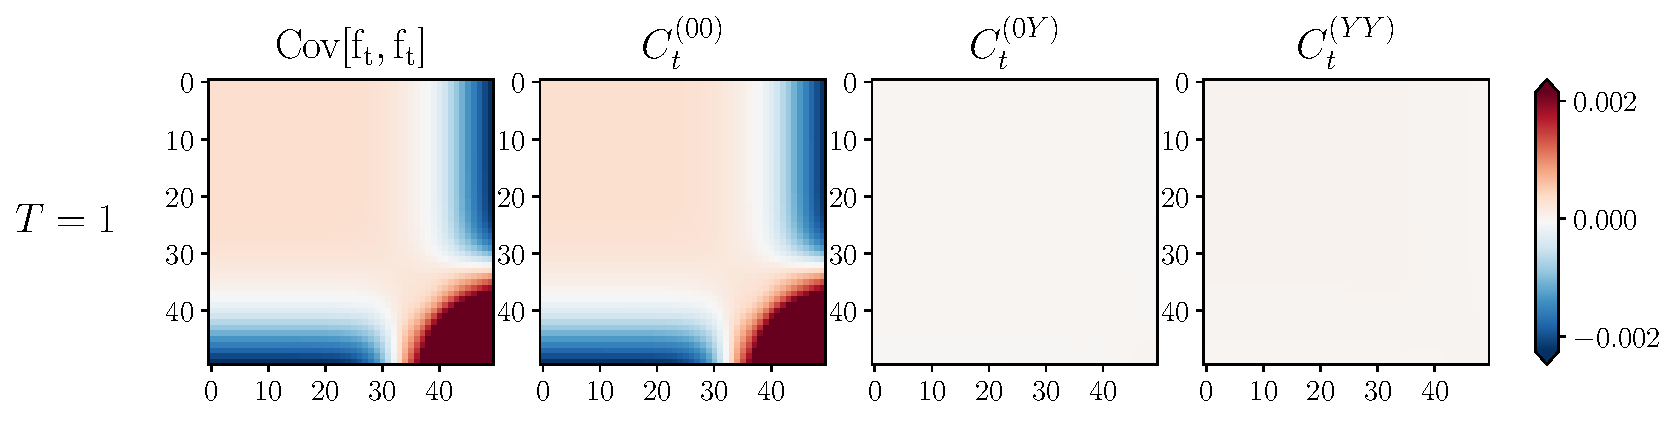
\includegraphics[width=0.90\textwidth]{plots/analytical_solution/covariance_ft_1_L0.pdf}
    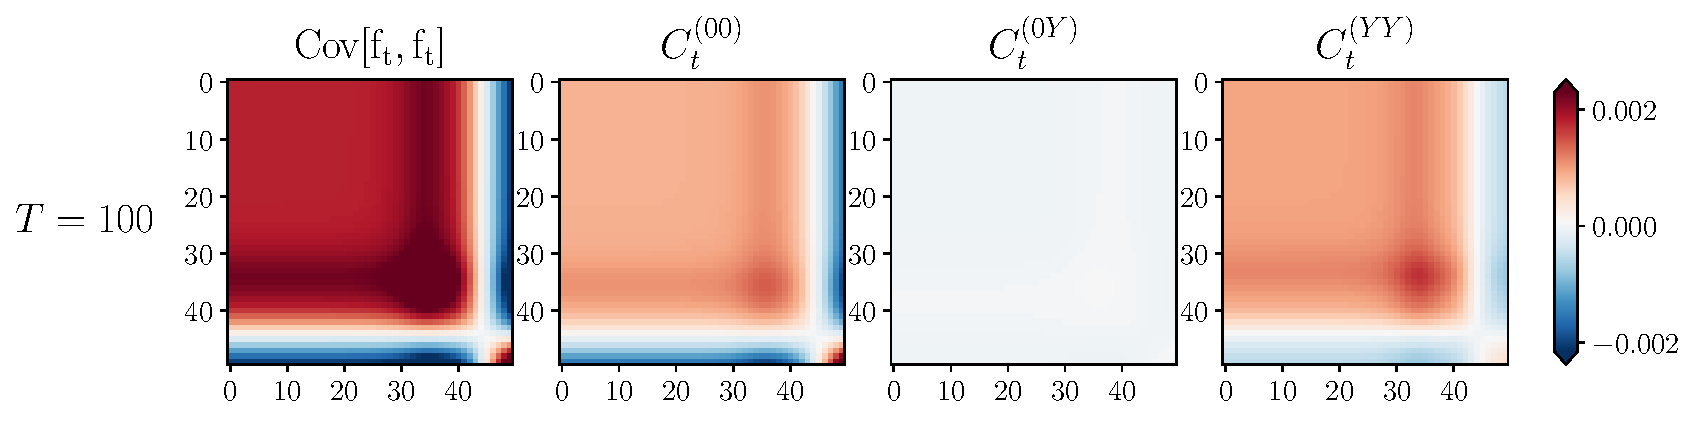
\includegraphics[width=0.90\textwidth]{plots/analytical_solution/covariance_ft_100_L0.pdf}
    \caption{Decomposition of the covariance of the trained solution, as
    described in Eq.~\eqref{eq:SumOfCovariances}, for different training epochs.
    The analytical solution is obtained by using a frozen NTK at
    $T_{\rm{ref}}=20000$ and the initial function $f_0$ is an ensemble of
    networks at initialisation different from the one used in the training
    process.}
    \label{fig:analytical_covariance_L0}
  \end{figure}
  % ===================================
  % L2
  % ===================================
  \begin{figure}[ht!]
    \centering
    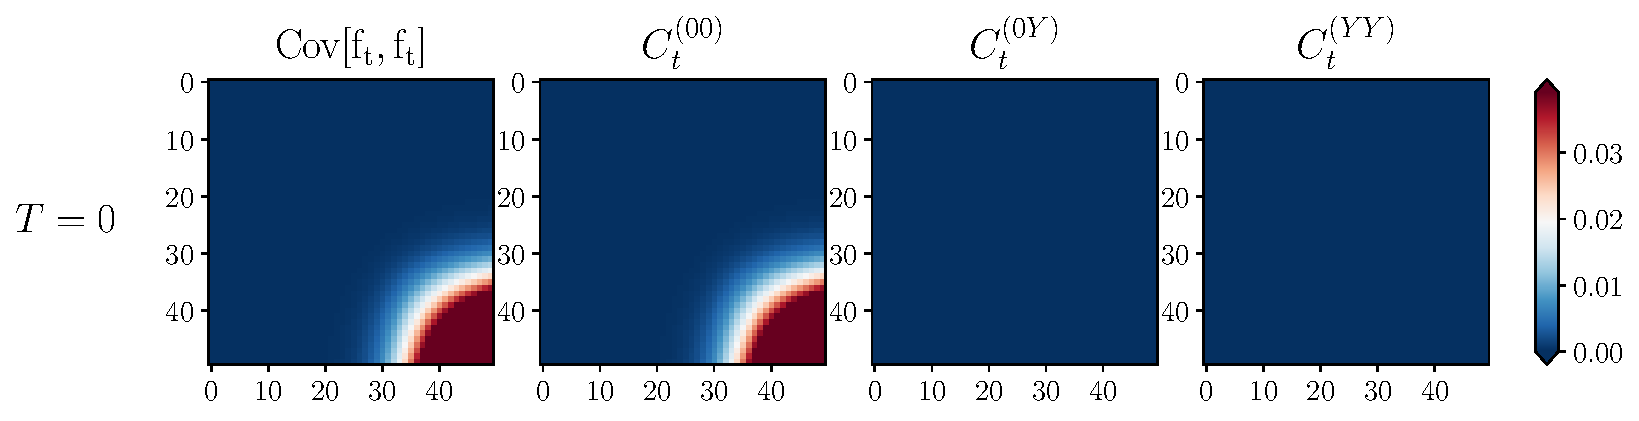
\includegraphics[width=0.90\textwidth]{plots/analytical_solution/covariance_ft_0_L2.pdf}
    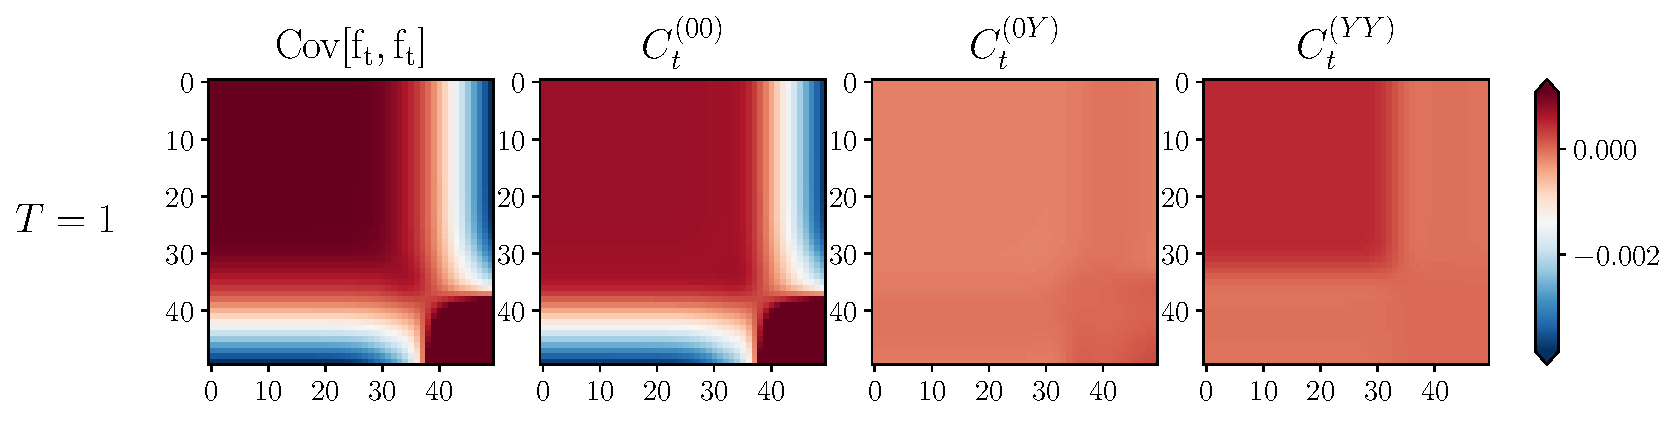
\includegraphics[width=0.90\textwidth]{plots/analytical_solution/covariance_ft_1_L2.pdf}
    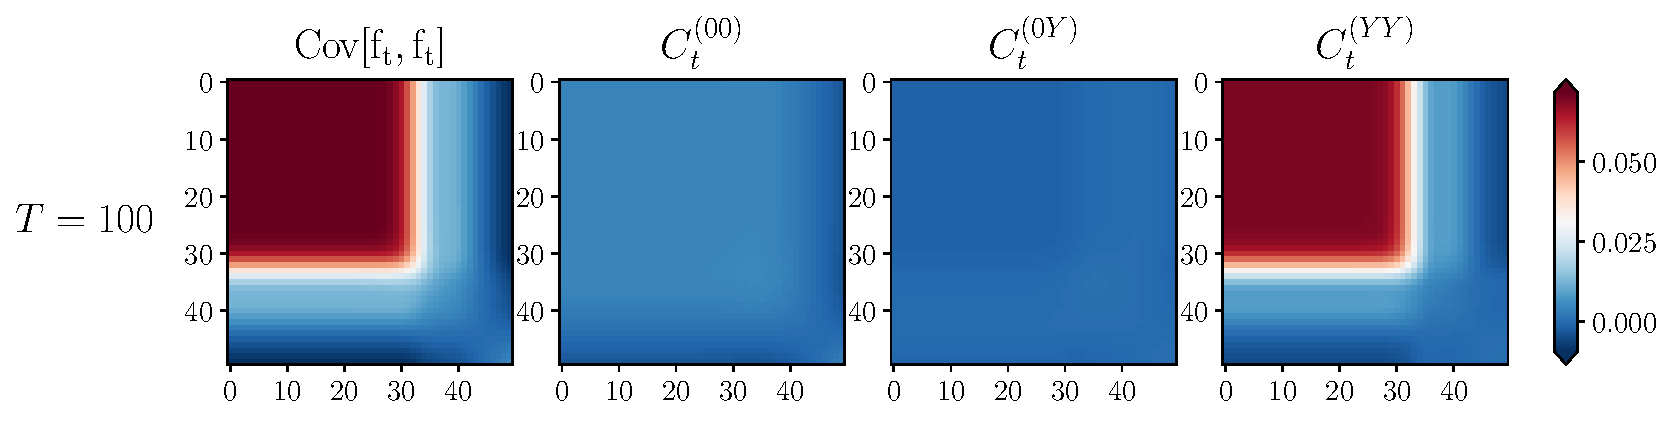
\includegraphics[width=0.90\textwidth]{plots/analytical_solution/covariance_ft_100_L2.pdf}
    \caption{Same as Fig.~\ref{fig:analytical_covariance_L0}, but for L2 data.}
    \label{fig:analytical_covariance_L2}
  \end{figure}
  % ===================================
For the covariance we have 
\begin{align}
    \cov[f_t,f_t^T]
        &= \mathbb{E}\left[U(t) f_0 f_0^T U(t)^T\right] 
            - \mathbb{E}\left[U(t) f_0\right] \mathbb{E}\left[f_0^T U(t)^T\right]  \nonumber \\
        &\quad + \mathbb{E}\left[U(t) f_0 Y^T V(t)^T\right] 
            - \mathbb{E}\left[U(t) f_0\right] \mathbb{E}\left[Y^T V(t)^T\right] \nonumber \\
        &\quad + \mathbb{E}\left[V(t) Y f_0^T U(t)^T\right]
            - \mathbb{E}\left[V(t) Y\right] \mathbb{E}\left[f_0^T U(t)^T\right] \nonumber \\
    \label{eq:CovAtT}
        &\quad + \mathbb{E}\left[V(t) Y Y^T V(t)^T\right]
            - \mathbb{E}\left[V(t) Y\right] \mathbb{E}\left[Y^T V(t)^T\right] \, .
\end{align}
Note that the first and the fourth lines above yield symmetric matrices, while the third line is just the 
transpose of the second, thereby ensuring that the whole covariance matrix is the sum of three symmetric 
matrices and therefore is symmetric, 
\begin{align}
    \label{eq:SumOfCovariances}
    \cov[f_t,f_t^T] = C_t^{(00)} + C_t^{(0Y)} + C_t^{(YY)}\, ,
\end{align}
where
\begin{align}
    \label{eq:C00term}
    C_t^{(00)} 
        &= \mathbb{E}\left[U(t) f_0 f_0^T U(t)^T\right] 
        - \mathbb{E}\left[U(t) f_0\right] \mathbb{E}\left[f_0^T U(t)^T\right]\, ,\\
    C_t^{(0Y)}
        &= \mathbb{E}\left[U(t) f_0 Y^T V(t)^T\right] 
        - \mathbb{E}\left[U(t) f_0\right] \mathbb{E}\left[Y^T V(t)^T\right] \nonumber \\
        \label{eq:C0Yterm}
        &\quad + \mathbb{E}\left[V(t) Y f_0^T U(t)^T\right]
            - \mathbb{E}\left[V(t) Y\right] \mathbb{E}\left[f_0^T U(t)^T\right] \, ,\\
    C_t^{(YY)}
        &= \mathbb{E}\left[V(t) Y Y^T V(t)^T\right]
        - \mathbb{E}\left[V(t) Y\right] \mathbb{E}\left[Y^T V(t)^T\right]\, .
\end{align}
The decomposition above is shown in Fig.\ref{fig:analytical_covariance_L0} for the L0 data and in
Fig.\ref{fig:analytical_covariance_L2} for the L2 data, where the three contributions of the covariance
are shown for different epochs.

\paragraph{Central value at infinite training time.}


\ldd{Move this to closure.}
We report the values of $C_t^{(00)}$, $C_t^{(0Y)}$ and $C_t^{(YY)}$ for different values of $t$ in 
Fig.\ref{fig:CovarianceContribs}.
\ldd{Here we need plots at many values of $t$, in order to figure out what is actually going on with these three 
contributions along training. Hoepfully we see explicitly that the fluctuations of the fields at initialization yield a 
contribution to the statistical uncertainty of the trained fields at early times, and that contribution
decreases.}

\begin{figure}[ht!]
    \centering
    
\includegraphics[scale=0.5]{plots/UoECentredLogo282v1160215.png}
    \caption{The various contributions to the covariance as described in the text above. 
    \ldd{Caption will change once we have the plot.}}
    \label{fig:CovarianceContribs}
\end{figure}

% % wrong limit
% In the limit where we ignore the fluctuations 
% of $U(t)$ and $V(t)$, we obtain
% \begin{align}
%     \cov[f_t,f_t^T]
%         &= \bar{U}(t) K \bar{U}(t)^T 
%             + \bar{V}(t) C_Y \bar{V}(t)^T\, ,
% \end{align}
% where we used the fact that the fluctuations of the data $Y$ are statistically independent from 
% the fluctations of the fields at initialization. 

\ldd{To be rewritten when we have the plots mentioned above.}

An important criterion that we want to put forward at this point is that the covariance of the trained
fields should be dominated by the statistical error on the data. This is the case towards the end of
training as shown in Fig.~\ref{fig:xT3_exp_val}. In this way we ensure that the quoted error 
on the PDFs is actually dominated by the statistical error on the data, and not by the fluctuations of the
initial fields. This is a crucial point, since it guarantees that the ensemble of trained PDFs is not biased by the
choice of prior that is made by selecting a given architecture, activation function, and probability distribution 
for the biases and weights at initialization. \ldd{More plots needed. To be discussed.}

\FloatBarrier
